\subsection{Notation}
Most of the notation is ``standard'' in the field of number theory and cryptography. Nonetheless, to avoid any misunderstandings and simplify some statements, we will present the notation used throughout the text. Anything that is not mentioned here shall be defined ``on the go'' with definitions and such. \\

\noindent Any scalars $a, t, \beta, \dots$ are represented by non-bold, latin or greek letters.\\
Bold symbols $\bm{v}, \bm{x}, \bm{s}, \dots$ will denote vectors. \\
$\alg{Algorithms}$ will be represented by $\alg{textsf font}$ names such as $\alg{Encrypt}$ or $\alg{Evaluate}$.\\
Traditionally, the symbols $\Z, \Q, \R, \C$ shall represent the sets of integers, rational, real and complex numbers, respectivelly.\\
Additionally, for any real $m \geq 0$, $\flo{m}$ shall denote greatest integer not exceeding $m$, $\round{m} = \flo{m + \frac{1}{2}}$ and $[m]$ is the set $\{1, 2, \dots, \flo{m}\}$.\\
%When the situation demands us to make use of many variables and/or indicies, we will be using Eisenstein notation which is defined as \krzys{fill that in}

\subsection{Lattices}
\subsubsection*{Basic definitions}
We define a \textit{lattice} as a discrete additive subgroup of $\R^n$. Once we fix a basis $\B = (\bm{b}_1, \dots ,\bm{b}_n) \in \R^n$ we can then describe the lattice as
\[ \Lambda = \mathcal{L}(\bm{B}) = \Bigl\{ \sum_i z_i \bm{b}_i : z_i \in \Z \Bigl\}.\]
In other words, $\Lambda$ is the $\Z$-span of the specific basis $\B$.

There are many bases for a lattice (actually, for $n \geq 2$, there are infinitely many as can be proven using a diagonalization argument), some ``better'' than others. This will be the foundation for some of the cryptosystems later like the GGH.

\begin{example}
    The simplest example of a lattice is the $\Z^n$ itself. Taking the standard basis $\B_1 = (\bm{e}_1, \dots, \bm{e}_n)$ we obtain
	\[ \mathcal{L}(\bm{B}_1) = \Bigl\{ \sum_i z_i \bm{e}_i : z_i \in \Z \Bigl\} = \Z^n. \]
\end{example}
More generally, $\Lambda$ is a lattice of rank $m$ in $\R^n$ if it is a rank $m$ free abelian group. Recall that we call a group \textit{free abelian group} of rank $m$ if it can be written as $\Lambda = \Z\beta_1 \oplus \cdots \oplus\Z\beta_m$ with $\beta_1, \dots, \beta_m$ linearly independent over $\R$ where $\oplus$ represents the direct sum. In this paper we will only consider lattices of full rank $n$. 

\begin{remark}
    We can also view the vectors $\bm{b}_i$ as the columns of the matrix $\B \in \R^n \cross \R^n$ in which case, our definition becomes:
    $$\Lambda = \mathcal{L}(B) = \{\bm{Bz} :  \bm{z} \in \Z^n \}.$$
\end{remark}

Reciprocally, any matrix $\bm{B} \in GL_n(\R)$ spans a lattice: the set of all integer linear combinations of its rows.

\begin{example}
\begin{enumerate}
    \item $\mathcal{L} = \begin{pmatrix}
        1 & 0\\
        0 & 1
	\end{pmatrix}$ in which case $\bm{b}_1 = \big(\begin{smallmatrix}
          1\\
          0
	\end{smallmatrix}\big)$ and $\bm{b}_2 = \big(\begin{smallmatrix}
          0\\
          1
        \end{smallmatrix}\big)$
    \item $\mathcal{L} = \{(z_1,z_2) : z_1 + z_2 \text{ is even}\}$
    \item $\mathcal{L} = \begin{pmatrix}
        1/3 & \pi\\
        0 & 21/7
        \end{pmatrix}$
\end{enumerate}
\end{example}

As noted before, the basis of a lattice is not unique. There is one that is particularly interesting to us, namely, the \textit{Hermite Normal Form} (HNF). A basis $\B$ is in HNF if it is upper triangular (or lower triangular - does not matter as long as one is consistent), all elements on the diagonal are strictly positive and any other element $\bm{b}_{i,j}$ satisfies $0 \leq \bm{b}_{i,j} < \bm{b}_{i,i}$.

\subsubsection*{Fundamental Domain}
\begin{definition}[Fundamental Domain] \label{fundamental}
    Let $\mathcal{L}$ be a lattice of dimension $n$ and let $(\bm{b}_1, \dots, \bm{b}_n)$ be a basis for $\mathcal{L}$. The \textit{fundamental domain} (or \textit{fundamental parallelepiped}) for $\mathcal{L}$ corresponding to this basis is the set
    $$ \mathcal{F}(\bm{b}_1, \dots, \bm{b}_n) = \{t_1\bm{b}_1 + \cdots + t_n\bm{b}_n : 0 \leq t_i < 1 \}.$$
\end{definition}

We define the \textit{volume} of $\mathcal{F}(\bm{B})$ as the volume of the corresponding parallelepiped in $\R^n$. The \textit{volume} -- closely connected to the determinant -- plays a very important role in our study which will become evident in later chapters. One of the advantages, of defining the fundamental domain, is that we can formalize the notion of area (or the determinant) of any given lattice. Recall that a lattice is just a countable collection of points and therefore has no volume by itself. This, however, is resolved by introducing the following.

\begin{definition}
    Let $\mathcal{L}$ be a lattice of dimension $n$ and let $\mathcal{F}(\bm{B})$ be a fundamental domain for $\mathcal{L}$ over some basis $\bm{B}$. We define the \textit{determinant} of that lattice as
	\[ \det (\mathcal{L}) = \VF{\bm{B}} = |\det (\bm{B}) | \]
\end{definition}

The next two propositions are arguably the two most fundamental resuls for lattice based cryptography. The first one, states that the $\det (\mathcal{L})$ does not depend on the choice of the basis for that lattice. The second, that our whole ambient space $\R^n$ can be described using only vectors from the lattice and the fundamental domain. We will only give an outline of the proofs for the sake of keeping this section compact. Full proofs, however, can be found in \cite{book}, chapter 6.4.

\begin{lemma}
    The $\det (\mathcal{L})$ of an $n$-dimensional lattice is invariant under the choice of the basis.
\end{lemma}

\begin{proof}[Outline of the proof]
    Let $\bm{B}_1, \bm{B}_2$ be two bases for a lattice $\mathcal{L}$. The crucial part of the proof is to note that any two bases are related by some unimodular matrix $U$ (i.e. a matrix with the determinant of $\pm 1$) s.t. $\bm{B}_1 = U \bm{B}_2$. Then it easily follows that 
	\[| \det (\bm{B}_1) | = \det (\mathcal{L}) = | \det (U \cdot \bm{B}_2) | = | \det(U) | \cdot | \det(\bm{B}_2) | = | \det(\bm{B}_2)| \]
\end{proof}

From now on we will write $\mathcal{F}$ to denote the fundamental domain of the lattice without specifying the basis.

\begin{proposition}
    Let $\mathcal{L} \subset \R^n$ be a lattice of dimension $n$ and let $\mathcal{F}$ be a fundamental domain for $\mathcal{L}$. Then every vector $\bm{v} \in \R^n$ can be written in the form 
    $$\bm{v} = \bm{f} + \bm{t}$$
    for $\bm{f} \in \mathcal{F}$ and $\bm{t} \in \mathcal{L}$ both unique and associated to the original $\bm{v}$.
\end{proposition}

Equivalently, the space $\R^n$ is spanned exactly (without overlap) by shifting the fundamental domain by the vectors from our lattice.
$$ \R^n = \bigcup_{\bm{t} \in \mathcal{L}} \{\bm{f} : \bm{f} \in \mathcal{F} \}$$

\begin{remark}
    Sometimes the \textit{fundamental domain} is refered to as a parallelepiped or parallelotope and denoted by caligraphic $\mathcal{P}$. If we take a matrix $\bm{B}$ to represent our lattice $\mathcal{L}$, then $\mathcal{P}_{1/2}(\bm{B}) = \{\bm{x}\bm{B}, \bm{x} \in [-1/2, 1/2]^n \}$ can also represent the (shifted by a half) fundamental domain of $\mathcal{L}$ (like for example in \cite{gentry}).
\end{remark}
\iffalse
We will now present two results that give us an upper bound on the length of the shortest vector in a lattice. This will later on be useful to determine the security and/or correctness of our schemes. These theorems are due to Hermite (1822 - 1901) and Minkowski (1864 - 1909).

\begin{theorem}[Hermite's Theorem]
    Every lattice $\mathcal{L}$ of dimension $n$ contains a nonzero vector $v \in \mathcal{L}$ satisfying
    $$ \norm{v} \leq \sqrt{n} \det(\mathcal{L})^{\frac{1}{n}}.$$
\end{theorem}
\krzys{add minkowski's theorem}\\
\fi
We can also need some notion of the shortest possible vector of a lattice. These will be very useful in the study of the hardness of a given problem.
\begin{definition}
	For a $n$-dimensional lattice $\Ll$, we denote its shortest nonzero vector (also called the \textit{minimum distance}) by $\lambda_1(\Ll)$. Formally
	\[ \lambda_1(\Ll) := \min_{0 \neq \bm{v} \in \Ll} ||\bm{v}|| \]
	More generally, for $1 \leq i \leq n$, the $i$th sucessive minimum of $\Ll$ is
	\[\lambda_i(\Ll) := \inf \{r : \Ll \text{ has $i$ linearly independent vectors of length at most } r \}. \]
\end{definition}
For example, in order to be able to go ``away'' from the lattice $\Ll$ ``out'' into the ambient space $\R^n$ and still be able to return to the original vector, we need to make sure the distance $d$ we travel is at most $\lambda_1(\Ll)/2$. This is for example a requirement in the \prob{BDD} problem where the decoding is \textit{promised}. For the exact definition see Section \ref{hardness}.

Aditionally, most of the problems used in this paper are the \textit{approximate} versions to some varying constant usually called $\gamma$. As we will see later, $\gamma$ very often depends on $\lambda_1(\Ll)$ which roughly measures how ``strict'' or ``precise'' we can make our problem. This will be made explicing in the Section \ref{hardness} on the hardness and complexity theory.

\paragraph{Dual}
\begin{definition}[Dual]
    For a lattice $\Ll \subset \R^n$ its $\Z$\textit{-dual} is
    \[ \Lld = \{ y \in \R^n : \langle y,\Ll \rangle \subseteq \Z \}.\]
\end{definition}

We simply require that the elements of the dual to be precisely those vectors, that yield an integer when ``multiplied'' with an element of our lattice. Note that this is different from our standard definition of a dual. Namely, it is not the orthogonal compliment of our starting space, i.e. not all of the elements of the dual have 0 dot product against the vectors of the lattice.

\begin{example}\label{ld-ex}
    Take $\mathcal{L}= \Z 
        \big(\begin{smallmatrix} 1\\2 \end{smallmatrix}\big) + 
        \Z \big(\begin{smallmatrix} 0\\ 1 \end{smallmatrix}\big)$.
        To calculate the dual of $\mathcal{L}$ we need our $y = \big(\begin{smallmatrix}
          a\\b\end{smallmatrix}\big)$ elements to satisfy $a +2b \in \Z$ and $b \in \Z$ which is equivalent to asking $a \in (1/2)\Z$ and so $\mathcal{L}^{\vee} = \big(\begin{smallmatrix}
          1/2\\0
        \end{smallmatrix}\big)\Z + \big(\begin{smallmatrix}
          0\\1
        \end{smallmatrix}\big) \Z$
        See Figure \ref{lattices} where the red vectors represent the basis.
\end{example}

Note that $\mathcal{L}^{\vee}$ is itself a lattice of the same dimension. One can imagine the dual as the original lattice ``flipped'' in the sence that the shortes element becomes the longest and vice versa.
\begin{figure}[ht]
    \caption{Lattice $\Ll$ from example \ref{ld-ex} and its dual.}
        \label{lattices}
        \centering
        \begin{subfigure}{.5\textwidth} 
                \centering
                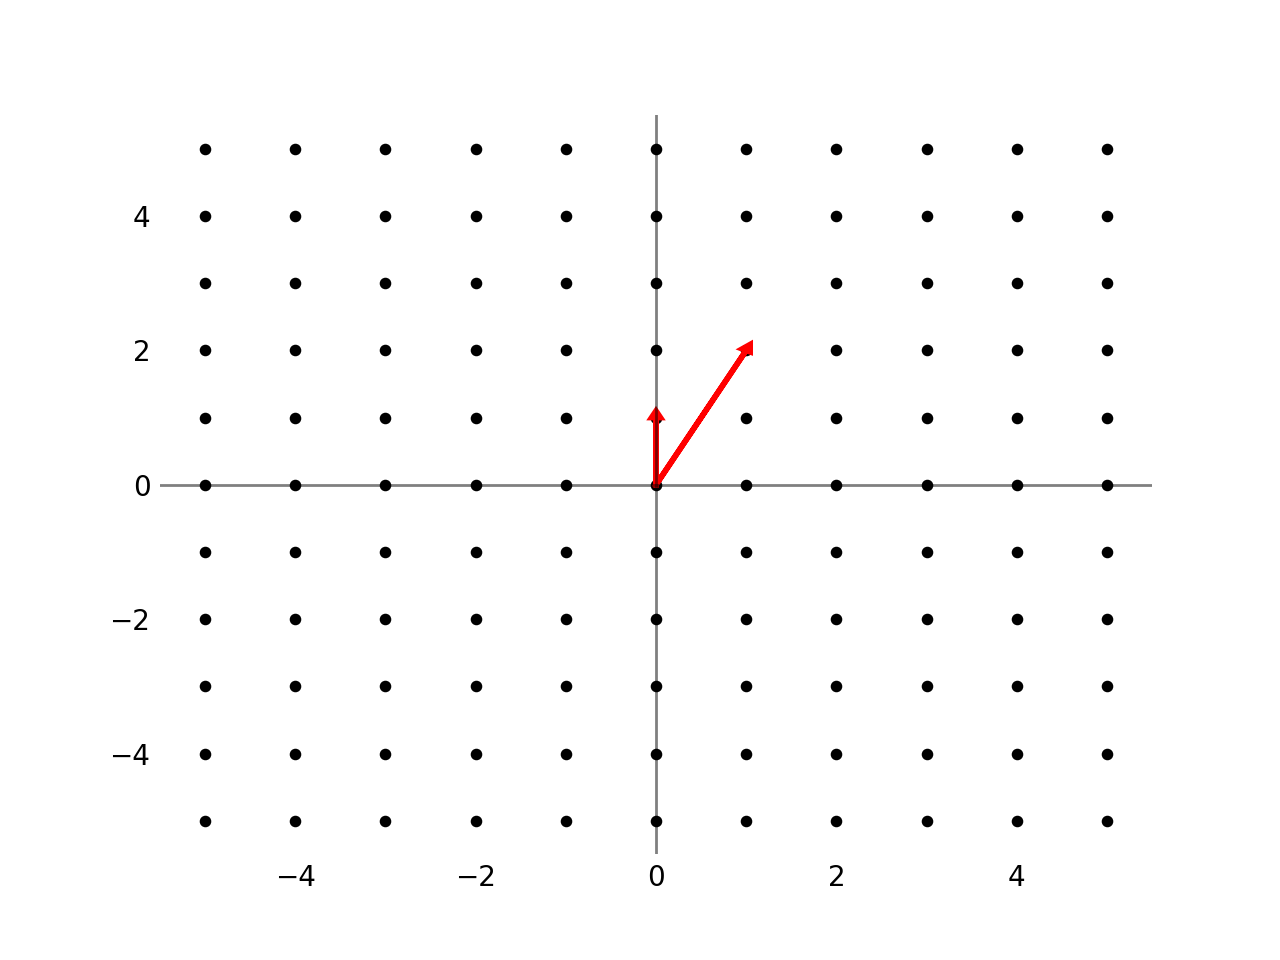
\includegraphics[scale=0.5]{lattice.png}
                \caption{$\Ll$}
        \end{subfigure}%
        \begin{subfigure}{.5\textwidth}
                \centering
                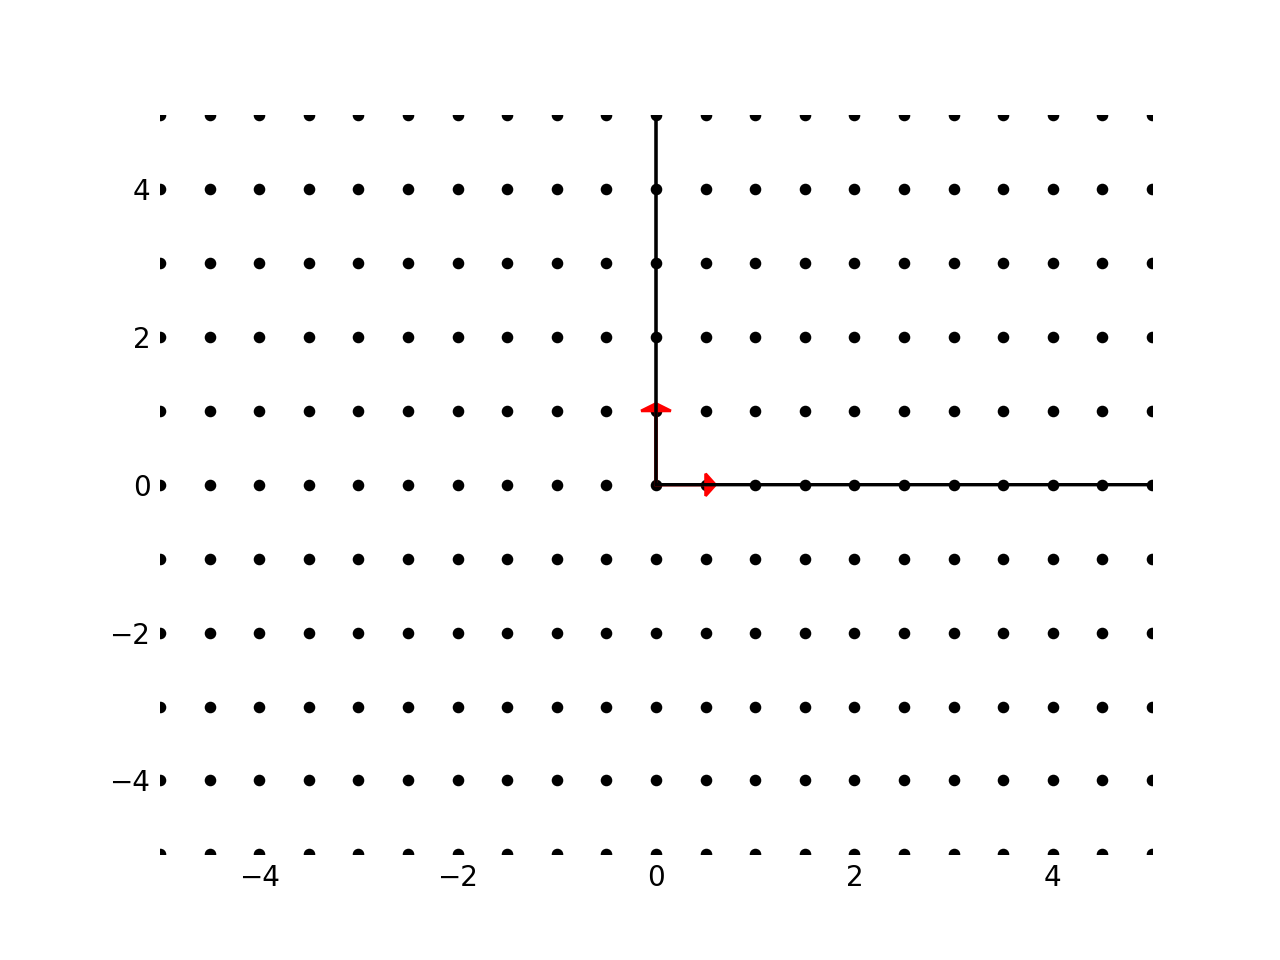
\includegraphics[scale=0.5]{lattice-d.png}
                \caption{$\Lld$}
        \end{subfigure}
\end{figure}

\subsection{Algebraic Number Theory}\label{ant}
Algebraic number theory is the study of \textit{number fields}, \textit{rings of integers} and \textit{finite fields}. In this section we will provide all the necessary background needed to understand and verify the results presented in the cryptographic schemes later in the text. Most results will be stated without proof however all of them can be found in the books like \cite{algebra} and \cite{ribenboim}.

\subsubsection*{Number Fields}
A \textit{number field} is defined as a subfield of $\oQ$ having finite dimension as a vector space over the rationals $\Q$. The \textit{degree} of a number field $K$ is defined as the dimension of $K$ over $\Q$ and when not stated otherwise, will be denoted by $n$. There exists a monic irreducible polynomial\footnote{Recall that we call polynomial monic if its leading coefficient is 1. It is an irreducible polynomial if it is irreducible as an element of the polynomial ring $\Q[x]$.} $f \in \Q[x]$ such that $K \cong \Q[x]/(f )$. In fact, every monic and irreducible polynomial in $\Q[x]$ defines a number field via such isomorphism.

\begin{definition}[Algebraic integer]
    An element $\alpha \in \C$ is an \textit{algebraic integer} if and only if, it is a root of some monic polynomial in $\Z[x]$.
\end{definition}
In fact, the set of \textit{algebraic integers} forms a ring.

\begin{definition}[Ring of Integers]
We define the \textit{ring of integers} (sometimes also called \textit{maximal order}) $\Oo_K$ of a number field $K$ as the intersection:
$$
  \Oo_K = K \cap \overline{\Z} = \{x \in K : \text{ $x$ is an algebraic integer}\}.
$$
\end{definition}

\begin{example}
    The field $K = \Q$ is a number field of degree 1. Its ring of integers is, as one can guess, the ordinary integers $\Z$.
\end{example}

\begin{example}\label{z-basis}
	The ring of Gaussian integers $\Z[\sqrt{-1}] = \{a+b\sqrt{-1}\, : \, a,b \in \Z \}$ is the ring of integers of $K = \Q(\sqrt{-1}) = \{a + b\sqrt{-1} \, : \, a,b\in \Q\}$ which has degree 2 since $x^2+1$ is the minimal (and irreducible) polynomial of $\sqrt{-1}$ over $\Q$. Note that $\Oo_K$ is spanned by $\{1, \sqrt{-1} \}$.
\end{example}

As another example, we can make a following statement about the ring of integers of a quadratic extension of rationals (real quadratic field).
\begin{lemma}
     Let $d \in \Z$ be a square-free integer. For the field $K = \Q(\sqrt{d})$, its ring of integers is 
     \[ \Oo_K = 
	 \begin{cases} 
	     \Z[\sqrt{d}] & \text{if $d \equiv 2, 3 \mod 4$}, \\
	     \Z[(1 + \sqrt{d})/2] & \text{otherwise}.
     	 \end{cases}
     \]
\end{lemma}

\begin{proof}
	Take $d \equiv 1 \mod 4$ square-free. \pinar{if you dont have time to finish the proof give a reference.}
\end{proof}
For example for $K = \Q(\sqrt{5})$ its ring of integers is $\Oo_K = \Z[(1 + \sqrt{5})/2]$. 
\begin{remark}\label{monogenic}
	What is worth noting here, is that for a number field $\Q(\alpha)$ for some $\alpha \in \oQ$, the ring of integers is not necessarily the $\Z[\alpha]$. Instead, $\Z[\alpha]$ is what's called an \textit{order} in $\Oo_K$. We will not consider them in general here because they are not relevant for our study as motivated in the next subsection. In general, a field $K = \Q(\alpha)$ such that $\Oo_K = \Z[\alpha]$ is called a \textit{monogenic} field or a \textit{simple algebraic extension}. For more details on orders, look at for example Chapter 5 of \cite{stein}.
\end{remark}

Recall that an ideal $\I$ of some ring $R$ is an additive subgroup of $R$ (if $x,y \in \I$ then $x-y \in \I$) and closed under multiplication of the elements in $R$ ($x \in \I$ implies $r \cdot x \in \I$ for any $r \in R$). We call an ideal in a ring of integers an \textit{integral ideal}.

One useful property of the integers we would like to preserve is the unique prime decomposition of its elements as stated in the Fundamental Theorem of Algebra. As the name might suggest\footnote{As stated on p.34 in \cite{stein} ``\textit{...it is this unique factorization that initially motivated the introduction of rings of integers of number fields over a century ago''}.}, the ring of integers has a property analogous to such decompositions. Namely, that every nonzero proper ideal factors uniquely into prime ideals. Such ring in general is called a \textit{Dedekind domain}.

More precisely, take $D$ to be a Dedekind domain (for example $\Oo_K$) and $\I \subset D$ a nonzero ideal (and also not an empty set). Then $\I$ factorizes uniquely (up to ordering) into prime ideals $\I = \p_1^{e_1} \p_2^{e_2} \ldots \p_r^{e_r}$ where each $e_i$ is an integer and each $\p_i$ is prime. Additionally it can be shown that in a Dedekind domain, every prime ideal $\p$ is also \textit{maximal}. This in turn implies that $D/\p$ is a finite field of order equal to the index of $|D /\p|$ as an additive subgroup of $D$.

As mentioned before, it is not in general true that $\Oo_K$ is a principal ideal domain. To mimic the notion of divisibility we will associate the elements of $\Oo_K$ with \textit{fractional ideals}.
\begin{definition}[Fractional ideal]
	A \textit{fractional} ideal of $\Oo_K$ is an ideal $\I$ of $K$ such that there exists some $\alpha \in \Oo_K$ such that $\alpha \cdot \I \subseteq \Oo_K$.
\end{definition}
The fractional ideals are genuine ideals of the field $K$ that were ``divided by something'', hence the name \textit{fractional}. We can also define their inverses as the set
\[ \I^{-1} = \{ \alpha \in K : \alpha \cdot \I \subset \Oo_K \}. \]

Therefore, the set of nonzero fractional ideals of $\Oo_K$ forms a group under multiplication with multiplication defined as $(\alpha \I)(\beta \J) := \alpha \beta \, \I \J$ and $\Oo_K$ itself acting as the identity element. %Since any (fractional) ideal $\I$ factorizes uniquely into prime ideals

\subsubsection*{Embeddings in $\C$} 
Let $K = \Q(\alpha)$ be a number field of degree $n$ for a root $\alpha$ of some irreducible $f \in \Q[x]$. It can be shown, that there are exactly $n$ embeddings (injective ring homomorphisms) of $K$ in $\C$. This can be shown noting that since $\Q$ has characteristic 0, all of the roots of $f$ over $K$ must be distinct. Therefore $\alpha$ can only be sent to any one of its $n$ conjugates over $\Q$. Each conjugate $\beta$ determines a unique embedding $\sigma_i: K \rightarrow \C$ and every embedding must arise in this way since $\alpha$ must be sent to one of its conjugates.

\begin{example}
    The quadratic field $\Q[\sqrt{d}]$, $d$ squarefree, has two embeddings in $\C$: The identity mapping, and also the one which sends $a + b\sqrt{d}$ to $a - b\sqrt{d}$ ($a$, $b$ $\in \Q$), since $\sqrt{d}$ and $-\sqrt{d}$ are the two conjugates of $\sqrt{d}$.
\end{example}
 
%As noted, we have many embeddings in $\C^n$. The simplest case could be the na\"ive coefficient embedding. Simply take an element of our number field $\alpha \in K = \Q[x]/(f)$ seen as a polynomial ring and map each of the coefficients $\alpha_i$ into the corresponding spot of the $\C^n$ vector. Although easy to picture, we will instead almost exclusively be using the \textit{canonical embedding} defined as follows.

\begin{definition}[Canonical embedding]
	Let $K = \Q(\alpha)$ be a simple algebraic extension (generated by just $\alpha$) of $\Q$ of degree $n$. Let $f(x)$ be the minimal polynomial of $\alpha$. Denote by $\sigma_i : K \rightarrow K$ the $\Q-$automorphism such that $\sigma_i(\alpha) = \alpha_i$ where $\alpha := \alpha_1$ and $\alpha_i$ are the roots of $f(x)$. The \textit{canonical embedding} $\sigma$ is defined as
	\[ \sigma : K \rightarrow \C^n, \; \; \; \alpha \mapsto  (\sigma_1(\alpha), \sigma_2(\alpha), \ldots, \sigma_n(\alpha)). \]
\end{definition}

\begin{example}
    For $K = \Q(\sqrt{5})$ we have two embeddings $a+b\sqrt{5} \mapsto a \pm b\sqrt{5}$ and so the cannonical embedding is given by
	\[ a + b\sqrt{5} \mapsto (a + b\sqrt{5},\, a - b\sqrt{5}). \]
\end{example}

One last thing we will need to introduce are the \textit{trace} of some field $K$.

\begin{definition}
	Let $K$ be a number field with $n = [K:\Q]$ and let $\sigma_1, \sigma_2, \ldots, \sigma_n$ denote the embeddings of $K$ in $\C$ just like above. For $\alpha \in K$ we define the \textit{trace} as
	\[ \Tr_{K/\Q}(\alpha) = \sum_{i \in [n]} \sigma_i(\alpha). \]
\end{definition}


\subsubsection*{Cyclotomic fields}
One particularly handy family of polynomials are the \textit{cyclotomic polynomials}. As defined momentarily, they are the minimal polynomials of the primitive roots of unity which poses many interesting algebraic properties. They also turn out to be much easier to compute and in general perform computational operations over, in contrast to most other polynomials.

\begin{definition}[Roots of unity]\label{r-of-1}
    Given a field $K$ and a positive integer $n$, an element $\zeta \in K$ is called \textit{primitive $n$-th root of unity} if $\zeta$ has order $n$ in the multiplicative group $K^{\cross}$. In other words, $\zeta^n = 1$ and $\zeta^k \neq 1$ for $1 \leq k < n$. 
\end{definition}
It is also true that all $\zeta^k$ for $1 \leq k < n$ and $\gcd(k,n) = 1$ are conjugates of $\zeta$. It follows that $\Q(\zeta)$ has degree $\varphi(n)$ over $\Q$. This leads us to the following proposition. Recall that the Galois group Gal$(K/\Q)$ of a finite extension of degree $n$ of $K$ over $\Q$ (or any other field for that matter) is the group of all $\Q-$automorphism. That is, Gal$(K/\Q)$ consists of maps $\tau : K \rightarrow K$ that fix $\Q$ elementwise. As a result the image of $\Q$ under $\tau$ is still $\Q$. 
\begin{proposition}[p. 13 in \cite{algebra}]\label{galois}
	The Galois group of $K = \Q(\zeta_n)$ over $\Q$ is isomorphic to the multiplicative group of integers$\mod n$
	\[ \Z_n^* = \{ k : 1 \leq k < n, \; \gcd(k,n) = 1 \}. \]
	For each $k \in \Z_n^*$ the corresponding automorphism in Gal$(K/\Q)$ sends $\zeta$ to $\zeta^k$.
\end{proposition}

The minimal polynomial $\Phi_n$ of $\zeta$ over $\Q$ is called the $n$-th cyclotomic polynomial. Formally we define it as 
\[ \Phi_n(x) = \prod_{\substack{\gcd(k,n) = 1 \\ 1 \leq k < n}} \bigg( x - \zeta^k \bigg) = \prod_{\substack{\gcd(k,n) = 1 \\ 1 \leq k < n}} \bigg( x - e^{2\pi k \sqrt{-1}/n} \bigg) \in \Z[x]. \]

The following equality is very useful for computing the polynomial itself:
\begin{equation}\label{comp_cycl} 
	\Phi_n(x) = (x^n - 1) \bigg/ \prod_{\substack{d | n\\ 1 \leq d < n}} \Phi_d(x) 
\end{equation}
\begin{example}
	To find $\Phi_8(x)$, we can use equation \ref{comp_cycl} to first precompute:
  \begin{align*}
	  & \Phi_1(x) = x - 1 \\
	  & \Phi_2(x) = x^2-1\Big/\Phi_1(x) = \frac{x^2 - 1}{x-1} = x+1 \\
	  & \Phi_4(x) = x^4-1\Big/\Phi_1(x)\cdot \Phi_2(x) = \frac{x^4-1}{(x-1)(x+1)} = x^2 + 1
  \end{align*}
	  And use it one more time to find:
	  \begin{align*}
		  \Phi_8(x) = \; & (x^8 - 1) \Big/ \prod_{{d | 4}} \Phi_d(x) = \Phi_1(x) \cdot \Phi_2(x) \cdot \Phi_4(x) \\
		  = \; & (x^8 - 1) \Big/(x-1)(x+1)(x^2+1) \\
		  = \; & (x^4+1)\cdot (x^2+1)(x+1)(x-1) \Big/(x^2+1)(x+1)(x-1) \\
		  = \; & x^4 +1,
	  \end{align*}
	  as desired.
\end{example}
As a useful corollary of the equation \ref{comp_cycl}, we can prove that for $n$ a power of 2, $n = 2^k$ for some $k \geq 1$, the cyclotomic polynomial $\Phi_n(x)$ is of the form $x^{2^{k - 1}} + 1$.
\begin{corollary}\label{2k-cycl}
  Let $n= 2^k$ for some $k \in \Z_{> 0}$. Then $\Phi_n(x) = x^{2^{k-1}} + 1$.
\end{corollary}
\begin{proof}
	We prove this by induction. We first check that indeed $\Phi_2(x) = x+1$. For the inductive step, assume that we have $\Phi_n(x) = x^{2^{k-1}} + 1$ for some $n = 2^k$. Then it is not difficult to see that $x^{2^k} -1$ ``splits'' as 
	\begin{align*}
		x^{2^k} = & (x^{2^{k-1}} + 1)(x^{2^{k-1}} - 1) \\
		= & (x^{2^{k-1}} + 1)(x^{2^{k-2}} + 1) \cdot \ldots \cdot (x+1)(x-1) \\
		= & (x^{2^{k-1}} + 1) \cdot \Phi_{2^{k-1}}(x) \cdot \ldots \cdot \Phi_2(x) \cdot \Phi_1(x) \\
		= & (x^{2^{k-1}} + 1) \cdot \prod_{d | n} \Phi_d(x)
	\end{align*}
	and so the equation \ref{comp_cycl} becomes
	\begin{align*}
		\Phi_n(x) = & (x^n - 1) \Big/ \prod_{d|n} \Phi_d(x) \\
		= & (x^{2^{k-1}} + 1) \cdot \prod_{d|n} \Phi_d(x) \Big/ \prod_{d|n} \Phi_d(x)\\
		= & x^{2^{k-1}} + 1
	\end{align*}
\end{proof}

As mentioned in Remark \ref{monogenic}, rings of integers are usually not generated by a single element. However, one very useful feature of cyclotomic fields is that their ring of integers is actually just $\Z[\zeta]$. That is -- $\Oo_K = \Z[\zeta]$ for $K = \Q(\zeta)$ and $\zeta$ is some $n$-th root of unity. This greately simplifies the approach in proving some of the results later in this paper as we will only need to look at what happens with $\zeta$ instead of all other generators.

\begin{proposition}\label{cycl-ok}
	The ring of integers of a cyclotomic number field $K = \Q[x]/\Phi_m(x) \cong \Q(\zeta)$ is $\Oo_K = \Z[\zeta]$. Additionally, if $n = \varphi(m)$ is the degree of $K$, then $\Z[\zeta]$ is generated by $\{1, \zeta, \zeta^2, \dots, \zeta^{n-1} \}$.
\end{proposition}

\begin{example}
		Similarly, for $K = \Q(\zeta_5) = \Q[x]/(x^4 +x^3 +x^2+x +1)$, we have four embeddings. These are precisely $\sigma_i(\zeta) = \zeta^i$ and now the canonical embedding maps $a + b\zeta + c\zeta^2 + d\zeta^3$ to
	\begin{align*}
		\begin{pmatrix}
		a + b\zeta + c\zeta^2 +d \zeta^3 \\
		a + b\zeta^2 + c\zeta^4 +d \zeta^6 \\
		a + b\zeta^3 + c\zeta^6 +d \zeta^9 \\
		a + b\zeta^4 + c\zeta^8 +d \zeta^{12}
		\end{pmatrix} = \begin{pmatrix}
		a + b\zeta + c\zeta^2 + d\zeta^3 \\
		a + b\zeta^2 + c\zeta^4 + d\zeta \\ 
		a + b\zeta^3 + c\zeta + d\zeta^4 \\
		a + b\zeta^4 + c\zeta^3 + d\zeta^2
		\end{pmatrix} = \\
		\begin{pmatrix}
		a + b\zeta + c\zeta^2 + d\zeta^3 \\
		a + d\zeta + b\zeta^2 + e\zeta^3 \\
		a + c\zeta + e\zeta^2 + b\zeta^3  \\
		a + e\zeta + d\zeta^2 + c\zeta^3 
		\end{pmatrix} = \begin{pmatrix} sth here
	\end{pmatrix}
	\end{align*}
	\krzys{i feel like i should get something nice but cant figure it our, its probs the $\zeta^4$}
\end{example}

In order to make $\sigma$ a ring homomorphism, we define the addition and multiplication in $\C^n$ to be coordinate-wise (all the conditions for a ring structure are immediate to see when written down because the $\C$ itself is a ring).

Another very handy property of the cyclotomic fields is that for $n > 3$, the $n$-th cyclotomic field has $\varphi(n)$ embeddings in $\C$. These are precisely the $\varphi(n)$ automorphisms where $\sigma_i(\zeta) = \zeta^i$ is simply the conjugation of the generator. Therefore $K$ has only complex embeddings and we call such field a CM-field. Since the $\Q$-automorphisms map $\zeta$ to one of its conjugates, it is easy to see that any automorphism $\tau_k : K \rightarrow K$ mapping $\tau_k(\zeta) = \zeta^k$ simply permutes the coordinates of the canonical embedding. More precisely, $\sigma_i(\tau_k(\zeta)) = \sigma_i(\zeta^k) = \zeta^{ik}$ for all $i,k \in \Z_{\varphi(n)}^*$. Hence $\sigma \circ \tau_k$ is just a permutation of the coordinates.

\subsubsection*{Ideal lattices}
Let us now get back to the topic of lattices for a moment and try to connect those two subjects a bit. Although not shown in this paper, we note that each element of $\Oo_K$ can be expressed as an integer linear combination of some basis $\bm{\mathcal{B}} = \{\beta_1, \beta_2, \ldots, \beta_n \} \subset \Oo_K$ (see the Exercise \ref{z-basis} as a simple case.). The set $\bm{\mathcal{B}}$ is also called the \textit{integral basis} of $\Oo_K$ and is also a basis for $K$ as $\Q$-vector space. Now recall from the beginning of the previous section that any lattice can be defined as the $\Z$-span of some specific basis $\mathcal{\bm{B}} \subset \R^n$. Analogously, we can define a lattice for any number field $K$.

\begin{definition}
	In a number field $K$ of degree $n$, a lattice in $K$ is the $\Z$-span of a $\Q$-basis of~$K$.
\end{definition}
Examples of lattices in $K$ include the ring of integers $\Oo_K$, fractional ideals of $\Oo_K$ and orders in $K$. By the unique decomposition, for any (fractional) ideal in $\Oo_K$, it can be shown that any such ideal is a free abelian group and is spanned by some $\Z$-basis $\{\beta_1, \beta_2, \ldots, \beta_n \}$. Therefore, under the canonical embedding $\sigma$, the ideal yields a rank-$n$ \textit{ideal lattice} with basis $\{\sigma(\beta_1), \ldots \sigma(\beta_n) \} \subset \C^n$. For convenience, we will often associate $\I$ with its embedding in $\C^n$ and talk for example about the shortest vector $\lambda_1(\I)$ of an ideal.

Analogously to the lattices in $\R^n$, we can define duals of lattices in $K$.
\begin{definition}
	Let $\Ll$ be a lattice in $K$. Its \textit{dual lattice} is
	\[\Lld = \{ \alpha \in K : \Tr_{K/\Q}(\alpha \Ll) \subset \Z \}.\]
\end{definition}
Imagine now, that we have some basis $\{1, \alpha, \ldots, \alpha^{n-1} \}$ for a number field $K = \Q(\alpha)$. If, in addition, $\alpha \in \Oo_K$ then the dual basis is characterized by the following proposition (this is special case of Theorem 3.7 in \cite{conrad}).
\begin{proposition}\label{d-basis}
	Let $K = \Q(\alpha)$ and let $f(x)$ be the minimal polynomial of $\alpha$ in $\Q[x]$. Then the dual basis to $\{1, \alpha, \ldots, \alpha^{n-1} \}$ (relative to the trace) is given by:
\[\biggl\{ \frac{1}{f'(\alpha)}, \frac{\alpha}{f'(\alpha)}, \ldots, \frac{\alpha^{n-1}}{f'(\alpha)} \biggr\} . \]
\end{proposition}
The lattice we will be most interested with is the ring of integers $\Oo_K$ itself. What can we say about $\Ood_K = \{ \alpha \in K : \Tr_{K/\Q}(\alpha \Oo_K) \subset \Z \}$? Firstly, it is the largest fractional ideal in $K$ whose elements all have trace in $\Z$ -- \cite{conrad}. The most important result for us however is how the dual of ring of integers ``controls'' every other fractional ideal $\I$.
\begin{proposition}
	For a fractional ideal $\I$ in K, $\I^{\vee}$ is a fractional ideal and $\I^{\vee} = \I^{-1} \Ood_K$.
\end{proposition}
\begin{remark}
The inverse of $\Ood_K$ is called the \textit{different ideal} and was first introduced by Dedekind in 1882 \cite{dedekind}. It has many interesting properties and we refer the curious reader to \cite{conrad} for more details about it as we will not mention anything else about it here.
\end{remark}








\subsection{Complexity Theory and Hard Problems} \label{hardness}
When talking about cryptography, we cannot avoid talking about algorithms since an encryption scheme is simply that, an instruction on how to encode sensitive data. We will thus require some terminology from computational complexity theory -- a field on the overlap of computer science and mathematics -- and cryptography. The problems the former field is concerned with are those of the time and space required for solving computational problems. Most of the time, the goal of the study is to prove the lower bound on the resources required to solve a problem using the best know algorithm. For example, how long does it take to find a factorization of a large composite number. The concern of the later -- cryptography -- is how to efficiently share secrets. The goal of this section is to give an overview of few parts of both fields which we will be using throughout the paper. 

\subsubsection*{Complexity theory}
We begin with necessary terminology. Throughout this section, $n$ shall denote the ``size'' of the input to the algorithm. Here the word ``size'' could mean many things like for example the bit-length of a number or its value in the base 10 representation.

In order to represent the time or space required to solve the problem, most of the time we will use the asymptotic notation of which the ``big-O'' is the most common. For any function $f$ and $g$ of some variable $n$, we say that $f(x) \in O(g(n))$ if there exists some constant $M > 0$ and $n_0$ such that $f(n) \leq Mg(n)$ for all $n \geq n_0$. Roughly speaking, the function $g$ will eventually ``grows faster'' than $f$. Variations on this notations include:

\begin{itemize}
	\item $f \in o(g)$ -- just like $O(g)$ but the inequality holds for all constants $M$. This provides more strict bounds as for example $2n = o(n^2)$ but $2n^2 \neq o(n^2)$ contrary to $2n^2 = O(n^2)$ (as well as $2n = O(n^2)$).
	\item The ``inverse'' of the small $o$ is $\omega$. Formally $f \in \omega(g)$ if for any $M$ there exists $n_0$ such that $f(n) \geq Mg(n)$ for all $n > n_0$. We call it the inverse of $o$ because $f(n) = o(g(n))$ if and only if $g(n) = \omega(f(n))$.
	\item $\tilde{O}(n) = O(n \ln n)$. That is, $\tilde{O}$ hides the logarithmic factors. For example, the FFT (Fast Fourier Transform) computes the discrete Fourier transform in time $O(n \ln n) = \tilde{O}(n)$ for a sequence of length $n$ and Shor's algorithm computes factorization of $n$-bit integer in time $O(n^2 \ln(n) \ln(\ln(n))) = \tilde{O}(n^2)$.
\end{itemize}

We will very often be talking about the ``efficiency'' of an algorithm. Intuitively, we want our procedure to run in a time reasonably proportional to the size of input. The consensus in the academia is to define ``efficient'' as running in polynomial time $\alg{poly}(n)$\footnote{As elegantly stated by Christos Papadimitiou: \textit{``It should not come as a surprise that our choice of polynomial algorithms as the mathematical concept that is supposed to capture the informal notion of ‘practically efficient computation’ is open to criticism from all sides. [$\ldots$] Ultimately, our argument for our choice must be this: Adopting polynomial worst-case performance as our criterion of efficiency results in an elegant and useful theory that says something meaningful about practical computation, and would be impossible without this simplification.''}}. More precisely, 
\begin{definition}
	An algorithm $A(n)$ is \prob{efficient} if there exists a polynomial $p(\cdot)$ such that the computation of $A(n)$ terminates within at most $p(n)$ steps.
\end{definition}
To encapsulate the notion of ``small'' or ``insignificant'', we define a \prob{negligible} amount in $n$ as an amount that is asymptotically smaller than $n^{-c}$ for any constant $c > 0$. More precisely, 
\begin{definition}\label{negl}
    $f (n)$ is a \prob{negligible} function in $n$ if 
	\[\lim_{n \to \infty}n^{-c} \cdot f (n) = 0\]
	for any $c > 0$.
\end{definition}

\subsubsection*{Hard problems}
The basis for modern day cryptography are so called ``hard problems'' of which usage was first formally introduced by S. Goldwasser and S.Micali in \cite{prob-cryp}. These are computational problems for which we do not know any efficient algorithm for (so far). The current approach to cryptography is to assume that some given problem is ``difficult'' to solve and then to prove that the scheme is secure given this assumption. The approach for the proof is to \textit{reduce} our scheme to the one we assume is hard. We proceed by showing how, an adversary, which is able to efficiently solve (or break) our scheme, is able to solve the underlying problem. We call such procedure a \textit{reduction} algorithm. For example, the basis for $\alg{RSA}$ is our inability to efficiently solve the factorization problem.
\begin{definition}[\prob{FACTORIZE}]
	Given a composite integer $n$ and $l < n$, find a non-trivial factor of $n$ less than $l$.
\end{definition}
In their paper \cite{rsa}, Rivest et. al. showed that ``\textit{[$\ldots$] breaking our system is at least as difficult as factoring $n$.''} which is precisely the idea behind a reduction algorithm. Another example of a hard problem would be the \textit{discrete logarithm problem} on which the Diffie-Helman key exchange protocol is founded.

Our schemes need to change soon however. In 1997, Peter Shor published a paper \cite{shor} showing a quantum algorithm that solves the above problem in polynomial time which, by our definition, is efficient. There are even more examples. As pointed out by Bernstein in \cite{bernstein} it turns out that number theoretic problems seem to be the place where quantum computers improve our algorithms the most. These include Pell's equation \cite{pell} or computing the unit group and class group of a number field \cite{17}, \cite{37}. This might however be due to our better understanding of number theory compared to any other basis for cryptography. We have been studying primes for centuries now but began looking into lattices only in late 19th century where the modern-day definition was introduced by Garrett Birkhoff in 1948 in \cite{birkhoff}.

Fortunately for us the best quantum computers are still in their infancy. The greatest integer factored using Shor's algorithm was 21 \cite{21} and it was done in 2012, eleven years after the famous Vandersypen et. al. experiment at IBM \cite{15} in which they factored the number 15. Nonetheless, we shouldn't wait until last minute and should therefore develop new schemes on problems for which we do not have any good (quantum) algorithms. One of the alternatives to number theoretic problems are lattices (among others like code-based or hash-based). Below we present few, most commonly used problems for lattices which will serve as a basis to prove hardness of our schemes.
\begin{definition}[$\gamma$-Shortest Vector Problem (\prob{SVP})]
	Given a basis for a lattice $\Ll$ of dimension $n$, find a nonzero vector $\bm{v} \in \Ll$ of length at most $\gamma \cdot \lambda_1(\Ll)$.
\end{definition}

\begin{definition}[$\gamma$-Shortest Independent Vector Problem (\prob{SIVP})]
	Like the SVP, except one outputs linearly independent $\bm{v}_1,\ldots , \bm{v}_n\in \Ll$, all of length at most $\gamma \cdot \lambda_n(\Ll)$.
\end{definition}
\begin{definition}[$\gamma$-Closest Vector Problem \prob{(CVP)}]
	Given a basis for a lattice $\Ll$ of dimension $n$ and a vector $\bm{t} \in \R^n$, output a nonzero vector $\bm{v} \in \Ll$ such that $\text{dist}(\bm{t,v}) \leq \gamma \cdot \text{dist}(\Ll, \bm{t})$.
\end{definition}

\begin{definition}[$\gamma$-Bounded Distance Decoding Problem (\prob{BDD})]
	Same as $\gamma$-$\alg{CVP}$, but with the promise that there is a unique solution -- i.e., we are given a lattice $\Ll$ and a vector $\bm{t} \in R^n$  (within distance $\gamma \cdot \lambda_1(\Ll)$ from the lattice), and we are asked to find a lattice point $\bm{v} \in \Ll$ within distance $\gamma \cdot \lambda_1(\Ll)$ from the target.
\end{definition}

We know that these problems are in fact NP-hard (for very small approximation factors) \cite{gentry}, \cite{bdd}. The best know algorithms are variations of LLL lattice reduction algorithm by Lenstra et. al. \cite{lenstra} or Babai's nearest plain algorithm \cite{babai}.

\begin{remark}
	We are still faced with a problem that is inherent to all of modern-day cryptography. That is, we are assuming the hardness of the problem based on our inability to efficiently solve it. As correctly trivialized by Daniel J. Bernstein \cite{bernstein}: ``\textit{nobody has figured out an attack so we conjecture that no attack exists}''. It might so happen that tomorrow someone finds an efficient (polynomial time) algorithm to find the shortest vector in a given lattice and our secrets are compromised. This is exactly what happened in the case of $\alg{RSA}$ cryptosystem when Shor found such efficient algorithm for integer factorization. There is not much we can do about it at least with our current approach to cryptography which is based on very precise complex-theoretic assumptions. This is because complexity theory does not provide any tools to prove that an efficient algorithm does not exist for any given problem.
\end{remark}

We will also sometimes use an \textit{oracle} in a reduction. An \textit{oracle} is an entity (we often treat is as a black box) capable of solving a problem (even undecidable ones can be used). An oracle appears automatically when we want to prove that a problem reduces to another. When we assume we are capable of solving some underlying problem, we name such algorithm an oracle and do not investigate what the actual implementation is.

\subsubsection*{Basic cryptographic concepts}
As the last part of this section, we will introduce few basic concepts that are often used in cryptography and that we mention at some point in this paper. The notions introduced here are very vague in order to keep this introduction compact. For more precise definitions see for example \cite{katz} Chapter 3.

The most fundamental of cryptographic concepts is what is called a \textit{one-way function}. This is a function $f$ that is relatively easy to compute for any input but near impossible to invert (i.e., find $m$ given $c = f(m)$). Almost all other constructions are based on such function and this is also how lattice-based cryptography emerged. In 1996 M.Ajtai presented \cite{ajtai} a one way function based on the problem of solving Short Integer Problems (SIS) which sparked interest of other researchers to work on what we call today the lattice-based cryptography.

\paragraph{Security}
When we talk about (quantum) \textit{security} of a scheme, we roughly mean that no one (not even quantum computer) is able to break the scheme in a polynomial-time with a non-negligible probability. By ``break'' we mean that they are not able to obtain a message $m$ from the ciphertext $c \leftarrow \alg{Encrypt}(m)$. This, most of the times, boils down to reducing the scheme to an underlying hard problem. Here we present few basic security notions that we mention along the way.

The most common type of security is the \textit{semantic security}. First formally introduced in \cite{prob-cryp}, was informally defined as ``\textit{[$\ldots$] whatever an eavesdropper can compute about the cleartext given the cyphertext, he can also compute without the cyphertext.''}. This means that whenever we are given a ciphertext $c$, that encrypts either $m_0$ or $m_1$ we are unable to tell which one it was, even if we were to chose between the two. More on that will appear in the chapter on fully homomorphic encryption.

\iffalse
\begin{figure}[hb]
	\centering
	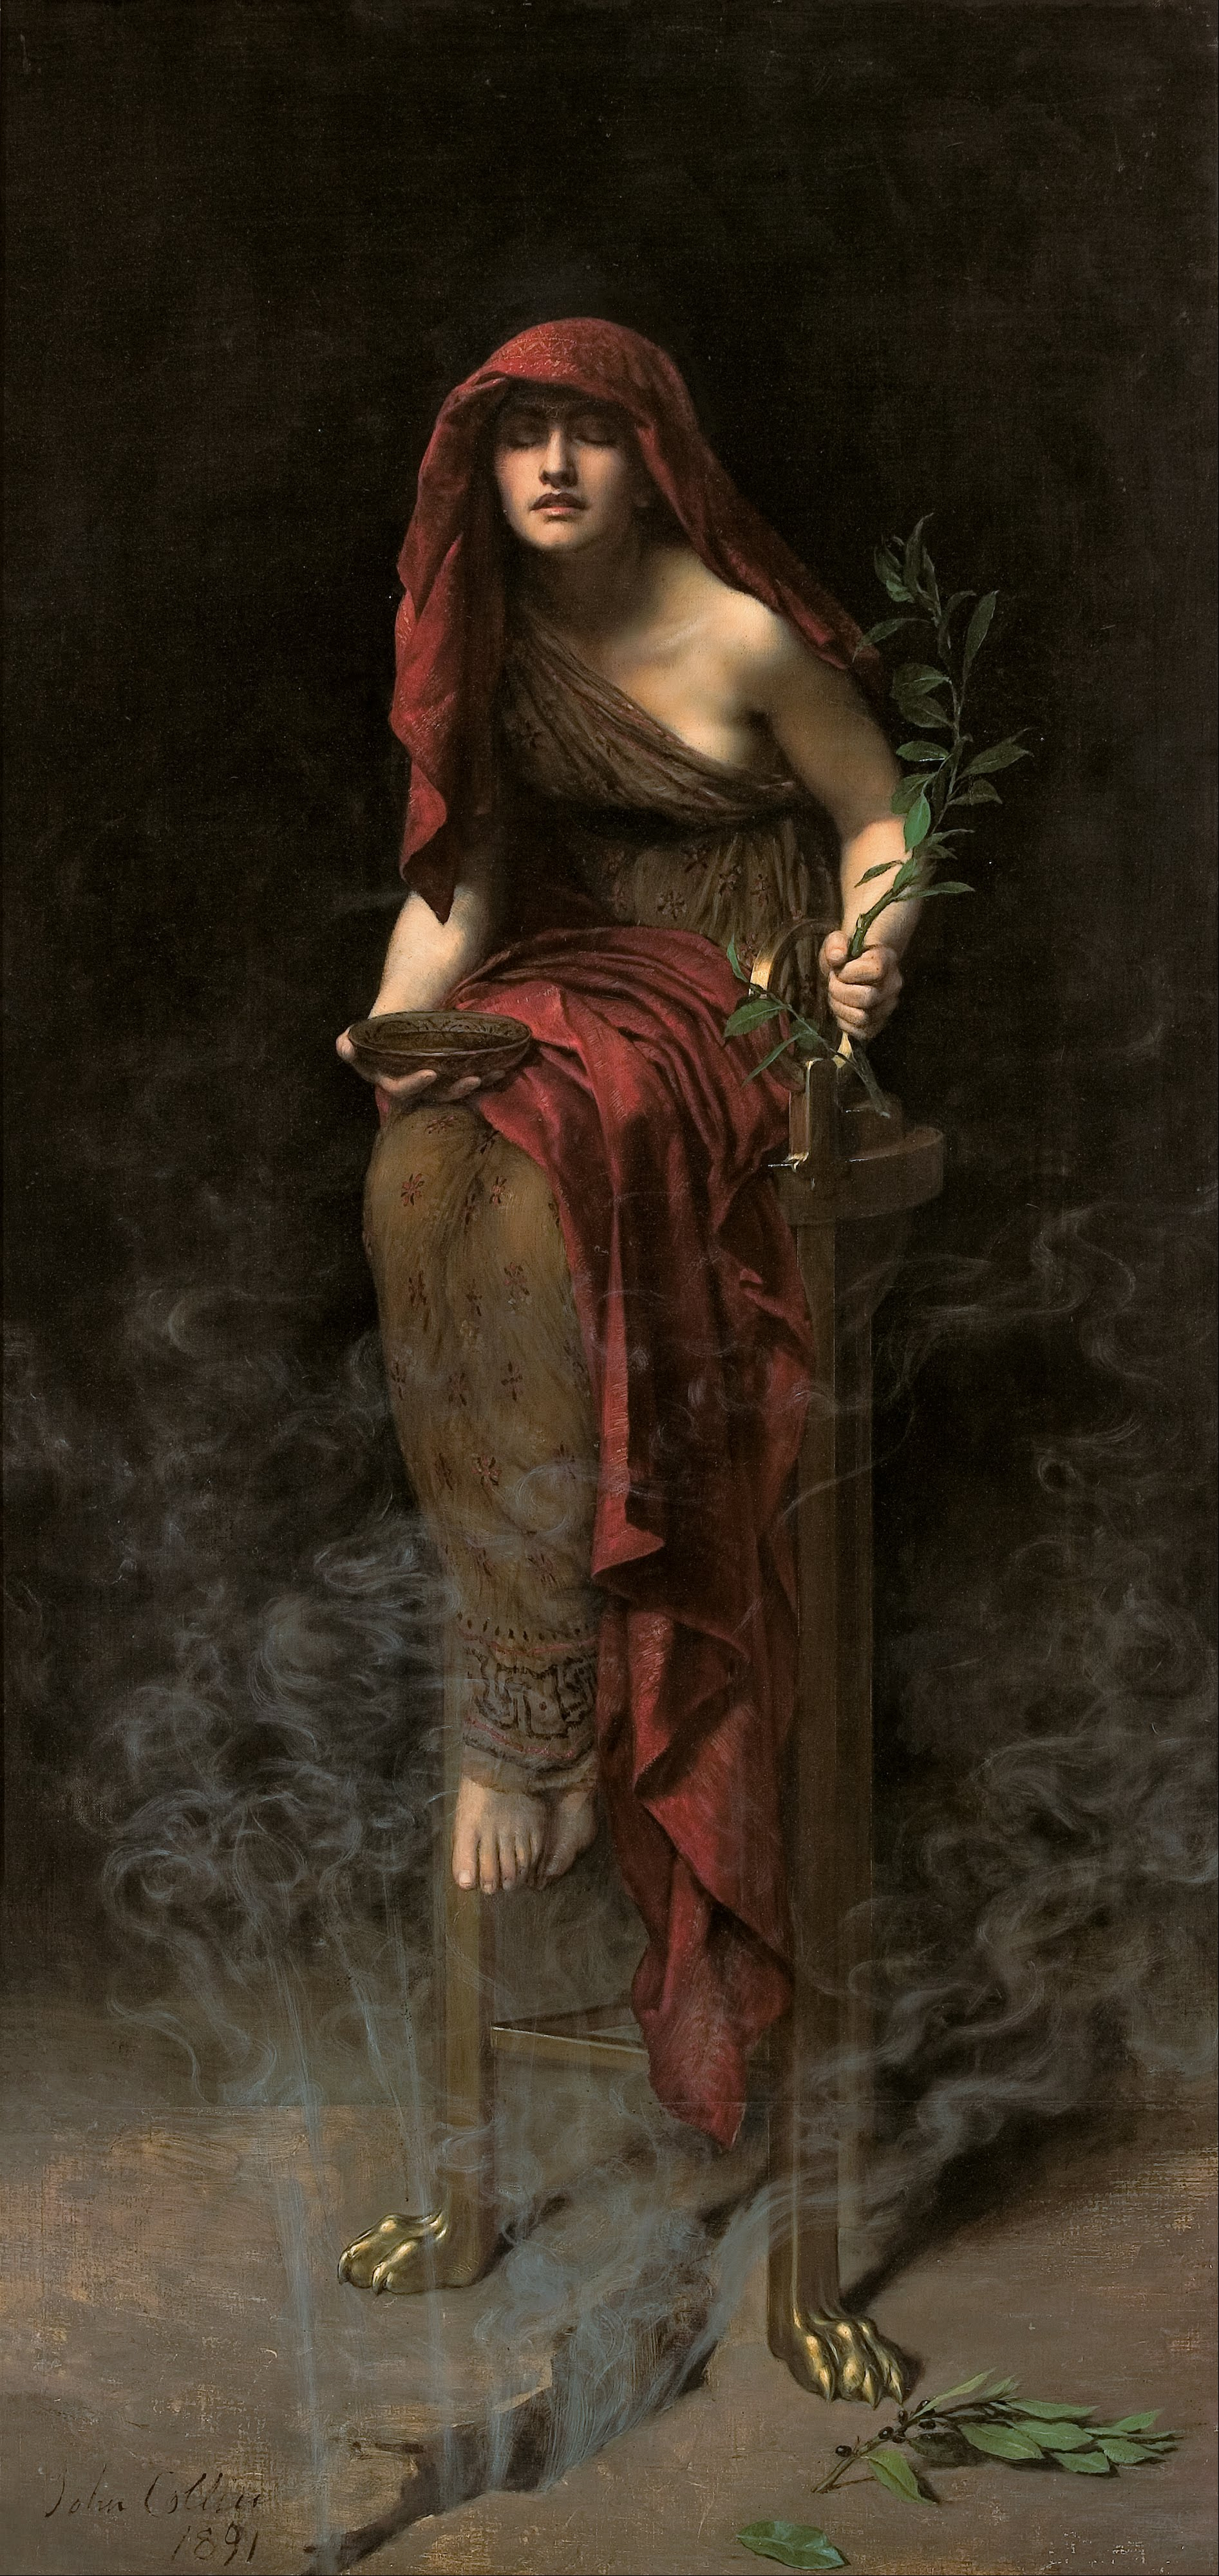
\includegraphics[width=0.3\textwidth]{pythia.jpg}
	\caption{Priestess of Delphi (1891) by John Collier.}
\end{figure}
\fi
